\subsection*{Questão 03}

\textit{Compare um sinal digital com um sinal analógico.}

\textbf{Resposta:}
\begin{itemize}
    \item \textbf{Sinal Analógico:} Varia continuamente no tempo e pode assumir qualquer valor dentro de um intervalo.
    É sensível a ruídos, pois qualquer pequena variação altera a informação.
    \item \textbf{Sinal Digital:} Varia em passos discretos e assume valores específicos.
    É mais robusto contra ruídos devido à regeneração de sinal e permite compressão/criptografia eficiente.    
    \item \textbf{Representação:}

    \begin{center}
        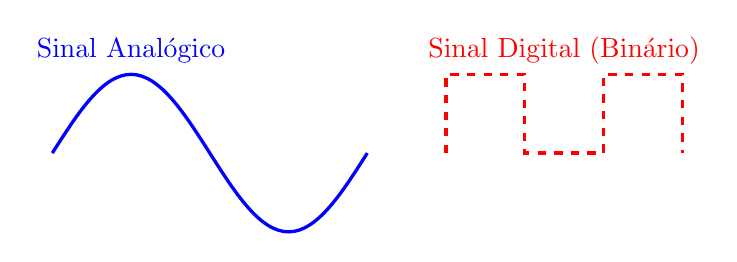
\begin{tikzpicture}
            \draw 
                [very thick, blue]
                (0, 0) sin (1, 1) cos (2, 0) sin (3, -1) cos (4, 0);
            \node[blue] at (1, 1.3) {Sinal Analógico};
            \draw
                [very thick, red, dashed]
                (5, 0) -- (5, 1) -- (6, 1) -- (6, 0) -- (7, 0) -- (7, 1) -- (8, 1) -- (8, 0);
            \node[red] at (6.5, 1.3) {Sinal Digital (Binário)};
        \end{tikzpicture}
    \end{center}
\end{itemize}